\label{sec:Intro}
There are many situations in which reference signals, or future disturbances are `previewable'. 
Optimal Preview Control is concerned with designing controllers that exploit previewed information in order to achieve performance levels that are superior to those achievable using current information alone. This paper considers the generic preview synthesis problem illustrated in Figure \ref{fig:DistRejSys}, which comprises a two-degree-of-freedom controller and both previewed disturbances/references ($r$), and unpreviewed disturbances ($w$).
An $\htwo$-optimal solution to this controller synthesis problem is provided that requires only low-dimensional computations and low-dimensional Riccati equation solutions, and leads to a controller whose high-dimensional component is a Finite Impulse Response (FIR) filter; the efficient implementation of FIR filters is well known is the signal processing literature.
The low-dimensional solution to the problem described in Figure~\ref{fig:DistRejSys} derives from the fact that the states of the (high-dimensional) delay line can be reconstructed by making a copy of $\Phi$ in the controller.  The objective of this paper is to provide a framework for synthesizing preview controllers for any problem that fits into the framework illustrated in Figure~\ref{fig:DistRejSys}. In addition, we aim to provide some general insights into the design of preview controllers, and a method for assessing the effectiveness of preview in terms of the achievable $\htwo$-norm reduction.
\begin{figure}
\begin{center}
\stdcontrolfrags
\psfrag{Phi}{$\Phi$}
\psfrag{r}{$r$}
\psfrag{rhat}{$\hat r$}
\psfrag{eta}{$\eta$}
\psfrag{G_p}{$G_p$}
\includegraphics[height=4.0cm]{./diags/DistRejSys.eps}
\caption{\label{fig:DistRejSys} A generalized regulator problem with both previewable and non-previewable disturbances. The transfer function $G$ is the system to be controlled, $K$ is the controller to be synthesized and $\Phi$ is an $N$-step delay line. The disturbance $w$ is not previewable, the control and measurement signals are $u$ and $y$ respectively, $\hat r$ is the previewable disturbance, and $r$ is the future value of $\hat r$. The filter $W_r$ is used  model the expected frequency content of $r$.}
\end{center}
\end{figure}

One of the first papers to recognise the importance of preview control is \cite{Sheridan}; three preview control models are described. In the third of these models open-loop optimal preview controls are found using dynamic programming. The earliest applied work on preview control dates back to \cite{Bender_1968_PrevSusp}, where Wiener filter theory was used to design an active suspension with road preview. Bender's solution required the transfer function from the previewed path to the vehicle's acceleration to be unstable --- such a solution is not implementable. Much of the subsequent work on preview tracking has its origins in the 1973 PhD thesis of M. Tomizuka~\cite{Tomi_1973_Thesis}, in which  the preview control task is cast in a discrete-time linear quadratic regulator framework by augmenting the plant dynamics with a delay line model. In this formulation the number of states grows in direct proportion to the preview length and so a direct solution of the corresponding Riccati equations becomes computationally infeasible for long preview lengths. Tomizuka presented an efficient recursive method for solving these large equations. A continuous-time version of a LQ preview control problem is studied in \cite{Tomizuka_1975_ContinuousLQPreview}, while a continuous-time preview control problem is given a stochastic interpretation in \cite{Lindquist}.

In the context of the early literature, \cite{Tomizuka_1975_OptDiscretePreview} provides a good overview of an output-feedback preview-tracking problem with reference noise. This paper also summarizes many of the basic properties of preview feedback controllers. 
Motivated by a process control problem, another previewable command reference variant, the so-called proportional, integral, derivative, preview (PIDP) controller is studied in \cite{Tomizuka_1979_IntegralPreviewFI} in an LQ optimal control framework. A closely associated feedforward problem is studied in \cite{Tomi_1980_FFPrev}. Other schemes for computing a feedforward-only controller is given in \cite{Zattoni_2006_H2PreviewFF} and \cite{Marro_2005_FFH2Preview}. Bender's vehicle suspension preview problem is re-visited in \cite{Tomi_1976_SuspRevisited} in a discrete-time command preview framework. The preview suspension problem has attracted the attention of several practitioners in the more recent literature; examples include \cite{Hac_1992_Opt_Veh_Susp,Marzbanrad_2004_SuspPrev,Roh_1999_Stoc_Opt_Prev,Sharp_2005_CarHandlingPreview}.

We will use the problem formulation in Figure \ref{fig:DistRejSys} as a basis for the results presented here. A solution will be derived
by formulating the problem in a generalised regulator framework \cite{LimebeerGreen,ZDG}, and then finding efficient solutions to the resulting high-dimension Riccati equations. Contributions made by this paper include:
\begin{itemize}
\item An efficient method for finding the $\htwo$ norm of the closed-loop system;
\item a method for evaluating the benefit of preview;
\item a low-order output feedback controller implementation;
\item an analysis of the  generic properties of preview controllers.
\end{itemize}

Figure~\ref{fig:SimpleSISOPrev} illustrates a simple example that may be used to highlight the benefit of preview, the broad structure of the controller, and the effect of preview on the achievable $\htwo$-norm of the closed-loop system. In this formulation, the preview action arises because of the delay line $\Phi$. The input to the controller is $r$, which is the future value of the reference, and $K$ is chosen so as to ensure that $e$ is `small', and hence the plant output follows $\Phi r$ as closely as possible. 
\begin{figure}
\stdcontrolfrags
\begin{center}
\includegraphics[width=0.4\hsize]{./diags/SimpleExampleNominalNoK2.eps}
\end{center}
\caption{A simple SISO open-loop preview tracking problem. The transfer function $\Phi=\z^{-N}$ is an $N$-step delay, $G$ is the plant to be controlled, and $K$ is a feedforward controller. The signal $r$ is the \textit{future} value of the reference, and $e$ is the tracking error.}
\label{fig:SimpleSISOPrev}
\end{figure}
%
First define the error system:
\als{E(\z)=G(\z)K(\z)-\Phi(\z),}
and assume that $G(\z)$ is stable; in the case that $G(\z)$ is unstable, it could be replaced by $\hat G(\z)=G(\z)(1-G(\z)K_f(\z))^{-1}$ in which $K_f(\z)$ is a stabilising feedback controller. Providing that $G(\z)$ has all its zeros inside the unit circle, perfect tracking ($E(\z)=0$) may be achieved by simply setting $K(\z)=G(\z)^{-1}\Phi(\z)$. 
However, if $G(\z)$ is {NMP}, then such a $K(\z)$ is not internally stabilising and a controller must be found that recognises the limits imposed by {NMP} zeros on the achievable tracking performance. %Such limitations are well known for non-preview systems (i.e. $N=0$ and $\Phi=1$), and are investigated in some detail in \cite{Middleteon_2004_PrevPerf} and \cite{Mirkin_2004_FixedLagPerfSaturation} for the preview case.

For the case where $G(\z)$ is an arbitrary stable, rational transfer function having a single real {NMP} zero at $c_z$, an algebraic expression for the $\htwo$-optimal controller will now be found. Our objective is to find an internally stabilising $K(\z)$ such that $\nrm{E(\z)}_2$ is minimised. 

The following inner-outer factorization  may be performed:
\als{G(\z)&= G_o(\z) G_i(\z),
\intertext{where: }
G_i(\z)&=\frac{\z-c_z}{1-\z c_z}
.}
We can write $E(\z)= (\tilde{K}(\z) -\Phi(\z)G_i(\z^{-1}))G_i(\z)$ in which $\tilde{K}(\z)= K(\z) G_o(\z)$ and:
\mbox{$G_i(\z^{-1})G_i(\z)=1$}. The optimal controller is found by setting $K(\z) = (\Phi(\z)G_i(\z^{-1}))_+ G_o^{-1}(\z) $, where $(\cdot)_+$ denotes the stable projection \citep{Doyle_1990_FeedbackControlTheory}. 
It follows by direct calculation  that:
\aln{K(\z)&=\underbrace{G_o(\z)^{-1}}_{IIR}\underbrace{\left(-c_z^{-1}\z^{-N} +  (1-c_z^{-2})c_z \sum^N_{i=1}(\z^{i-N}/c_z^i) \right)}_{FIR},\nonumber
\intertext{and that:}
\nrm{E(\z)}_2&=\frac{1}{\left|c_z^{N+1}\right|}\sqrt{c_z^2-1}.\label{eqn:H2normsimple}}
%


 
Since $\nrm{E(\z)}_2\rightarrow 0$  as $N\rightarrow \infty$, we conclude that in this example preview action can overcome completely the tracking limitation
imposed by the {NMP} zero. The optimal controller contains a high-order {FIR} part and a low-order {IIR} part, where the preview action comes from the {FIR} part. The dynamics of the {FIR} block is  fully specified by the {RHP} zero, $c_z$, and the preview length, $N$. The fact that the high order part of the controller is FIR leads to an efficient hardware implementation.
%A similar structure is also observed in the solution to the synthesis problem of Figure~\ref{fig:DistRejSys}, and leads to an efficient implementation of the high-order controller. 

A pole-zero plot of the optimal controller is given in Figure \ref{fig:PZforSISOPrevH2} for the case where $c_z=1.05$, $G_o(\z)=(1-\z c_z)/(\z-0.5)$, and $N=20$. Notice the almost pole-zero cancellation on the real axis. In the limit $N\rightarrow \infty$ cancellation occurs. 
\begin{figure}
\begin{center}
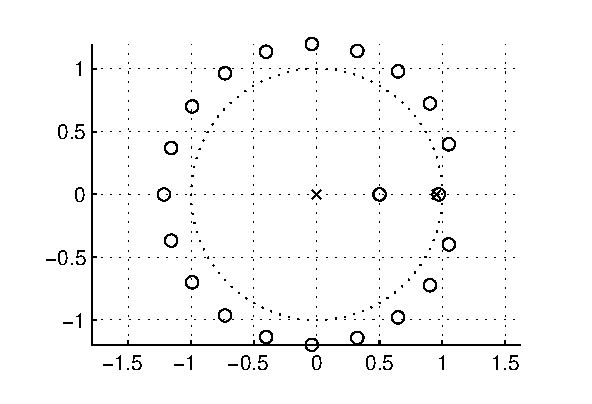
\includegraphics[width=0.7\columnwidth]{./diags/SimpleExamplePZPlot2.eps}
\end{center}
\caption{Pole-zero plot of the $\htwo$-optimal $K(\z)$ for the case where $c_z=1.05$, $G_o(\z)=(1-\z c_z)/(z-0.5)$ and $N=20$.   }
\label{fig:PZforSISOPrevH2}
\end{figure}
This simple preview problem highlights several important features that will be carried over into the more complex problem treated in this paper. In particular:
\begin{enumerate}
\item The preview action is captured in an {FIR} block having order $N$.
\item The remainder of the controller (the {IIR} part) has order equal to the plant order.
\item The preview length (N) required to achieve 95\% (for example) of the maximum norm reduction due to preview, is affected by the position of {NMP} zeros. 
\end{enumerate} 

Point 3 merits further discussion. A central tenet of this paper is that the preview length could be sufficiently large that solution of the associated {DARE} is computationally intractable. However, it might be argued that it is never necessary to use a large preview length because one could simply reduce the sampling rate until $N$ becomes sufficiently small.  In \cite{Middleteon_2004_PrevPerf}, a similar example is treated in continuous-time and it is found that the required preview \textit{time} is purely a function of the position of the continuous-time zero. The discrete-time equivalent is: for a given performance improvement, the preview time $NT_s$ (where $T_s$ represents the sample time) is determined by the position of the continuous-time zero. This fact can be seen by considering the effect of $T_s$ on the magnitude of $c_z$ in (\ref{eqn:H2normsimple}). Typically, the sampling rate is determined by the frequency at which tracking or disturbance rejection is required, and also by the frequency of any unstable poles \citep{Houpis_1991_DigitalControlSystems}. It therefore follows that a combination of low frequency zeros (which impose a large $NT_s$), and higher frequency performance specifications (which impose a low $T_s$), would lead unavoidably to a large preview length ($N$).% in order to achieve 95\% of the maximum available benefit due to preview.

%An obvious conclusion to be drawn from the example in this section is that preview is potentially useful when designing feedforward controllers for {NMP} systems. However, if one has a control problem with an unstable plant, which is stabilised by a feedback controller, then the resulting closed-loop will often be {NMP}, and so preview action is also potentially useful when controlling unstable systems.

At this stage, the reader might be left with the impression that preview is of no benefit for {MP} plants. However, as an example, it can be shown that the minimum achievable $\htwo$-norm of the transfer function:
\als{
\ma{E(\z)\\\rho K(\z)}
,}
is reduced by preview action, even when $G(\z)$ is {MP}. By adding the additional term $\rho K(\z)$ into the optimisation,
we are effectively penalising the magnitude of the control action. In general, a large $\rho$ leads to a slow response and so a large $N$ is required in order to get the full benefit from preview action. A detailed analysis of the effects of preview on systems of this form is given in \cite[Chapter 4]{Hazell_2007_Thesis}

The paper is structured as follows: Preliminaries and some standard notation is given in Section~\ref{sec:notation}. A state-space description of the generalized regulator problem with both previewable and non-previewed exogenous disturbances is derived in Section~\ref{sec:Sys}. The solution of this problem, which is illustrated in Figure~\ref{fig:DistRejSys}, is the central focus of the paper. Following a summary of the general theory, the full-information preview control problem is solved in Section~\ref{sec:H2FI}. The results are mainly concerned with efficient algorithms for solving the $\htwo$ full-information Riccati equation, and the evaluation of the full-information feedback gain matrix. The solution of the output feedback preview problem is given in Section~\ref{sec:H2OF}. The output feedback controller involves a combination of a state-estimator, and the solution to the full-information problem. An efficient controller synthesis is also given in this section. The effect of preview in reducing the $\htwo$-norm of the closed-loop system is analysed in Section~\ref{sec:2norm}. The special case of feedforward control with preview is analysed in Section~\ref{sec:Preproc}. A summary of the main features of preview controllers, as well as some design insights, are given in Section~\ref{sec:H2PrevSum}. The conclusions are given in Section~\ref{sec:Conclusions}.